\textcolor{black}{\section{Resultados y Análisis}}

\subsection{PARTE 1}
\noindent

\subsection{PARTE 2}
\noindent Con las mediciones hechas de forma manual se obtuvieron las gráficas de las Figuras \ref{Graf:2v_manual}, \ref{Graf:3v_manual} y \ref{Graf:4v_manual}.

\begin{figure}[H]
	\centering
	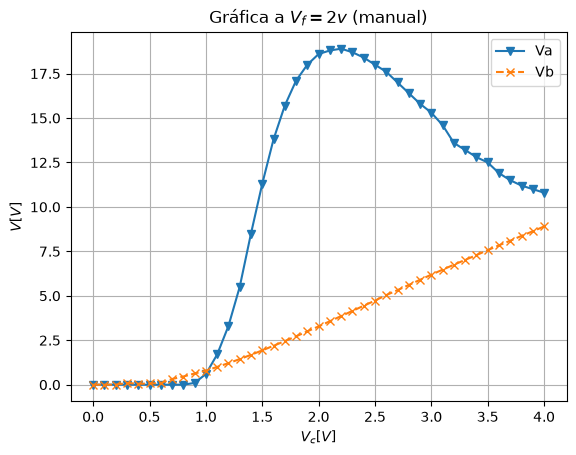
\includegraphics[scale=0.4]{figs/part2-2v_manual.png}
	\caption{Gráfica del voltaje del ánodo y del voltaje de la rejilla-blindaje registradas por el multímetro  contra el voltaje del cátodo a un voltaje fuente de $2\,V$.}
	\label{Graf:2v_manual}
\end{figure}

\begin{figure}[H]
	\centering
	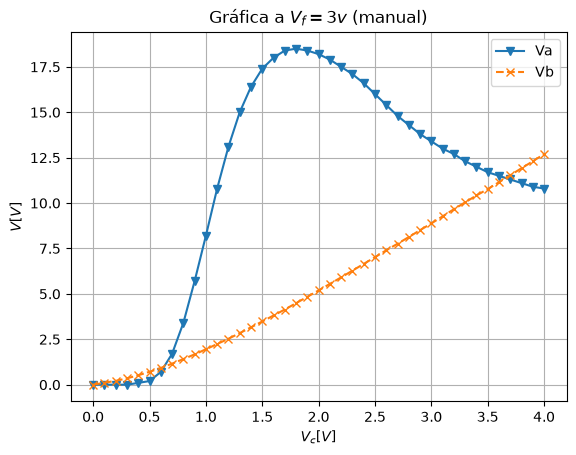
\includegraphics[scale=0.4]{figs/part2-3v_manual.png}
	\caption{Gráfica del voltaje del ánodo y del voltaje de la rejilla-blindaje registradas por el multímetro  contra el voltaje del cátodo a un voltaje fuente de $3\,V$.}
	\label{Graf:3v_manual}
\end{figure}

\begin{figure}[H]
	\centering
	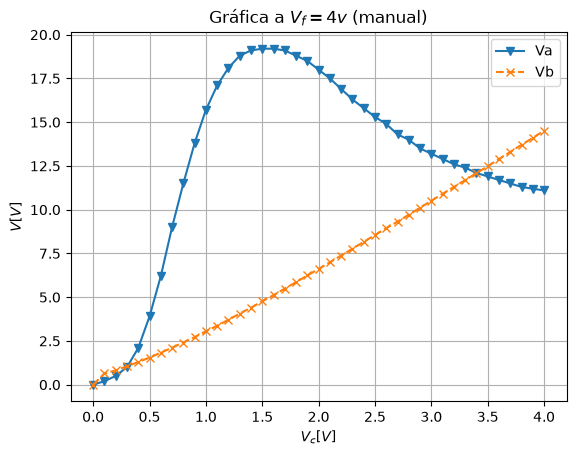
\includegraphics[scale=0.4]{figs/part2-4v_manual.png}
	\caption{Gráfica del voltaje del ánodo y del voltaje de la rejilla-blindaje registradas por el multímetro  contra el voltaje del cátodo a un voltaje fuente de $4\,V$.}
	\label{Graf:4v_manual}
\end{figure}

Como podemos ver de las graficas  \ref{Graf:2v_manual}, \ref{Graf:3v_manual} y \ref{Graf:4v_manual} existe una tendencia de $V_a$ de aumentar rápidamente y posteriormente desciende gradualmente, esto se debe a que $V_c$ define la energía cinética con la que los electrones atraviesan el gas, por lo que existe una sección de mínima dispersión, y una vez que se llegar a al máximo de la sección eficaz es tanta la energía cinética de los electrones que aumenta las colisiones de estos por lo cual disminuye de nuevo.

También podemos observar que al cambiar $V_f$ la sección eficaz  se recorre a la izquierda esto se debe a que si aumentas $V_f$ los electrones salen con mayor energía por eso necesitan menor $V_c$, también se debe a que se crea un nube de electrones en el cátodo, la cual crea su propio potencial eléctrico que acelera a los electrones, entonces si se aumenta el $V_d$ también aumenta la nube de electrones.

Las graficas realizadas de las mediciones hechas por el software del laboratorio se pueden observar en las Figuras \ref{Graf:2v_automatic}, \ref{Graf:3v_automatic} y \ref{Graf:4v_automatic}.

\begin{figure}[H]
	\centering
	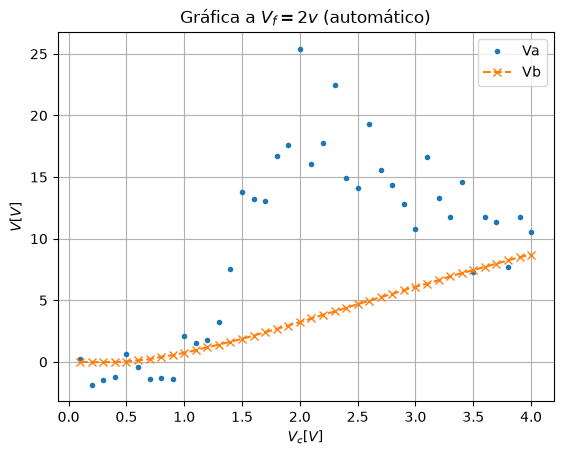
\includegraphics[scale=0.4]{figs/part2-2v_automat.png}
	\caption{Gráfica del voltaje del ánodo y del voltaje de la rejilla-blindaje registradas por el software del laboratorio contra el voltaje del cátodo a un voltaje fuente de $2\,V$.}
	\label{Graf:2v_automatic}
\end{figure}

\begin{figure}[H]
	\centering
	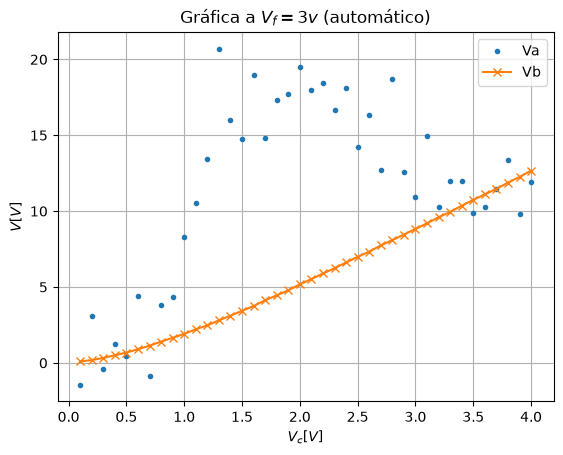
\includegraphics[scale=0.4]{figs/part2-3v_automat.png}
	\caption{Gráfica del voltaje del ánodo y del voltaje de la rejilla-blindaje registradas por el software del laboratorio contra el voltaje del cátodo a un voltaje fuente de $3\,V$.}
	\label{Graf:3v_automatic}
\end{figure}

\begin{figure}[H]
	\centering
	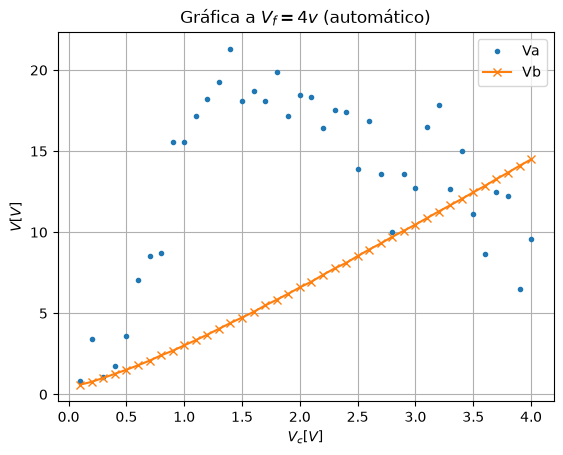
\includegraphics[scale=0.4]{figs/part2-4v_automat.png}
	\caption{Gráfica del voltaje del ánodo y del voltaje de la rejilla-blindaje registradas por el software del laboratorio contra el voltaje del cátodo a un voltaje fuente de $4\,V$.}
	\label{Graf:4v_automatic}
\end{figure}

Al observar los dato obtenidos de manera automática, podemos ver de las graficas  \ref{Graf:2v_automatic}, \ref{Graf:3v_automatic} y \ref{Graf:4v_automatic}, que existe una gran dispersión en el $V_a$ esto se debe a que el software tomo los datos al instante después de cambiar el $V_c$ y no espera a que el voltaje de diodo se estabilizara.  
